This year’s tournament challenges involved quite some non-verbal user interaction such as detecting to what object the user was pointing at. In the previous section the way we do people recognition is explained. This recognition includes information about the posture of each 3D skeleton. Once the people information is inserted into the world model, additional properties can be added to the persons that take also other entities in the world model into account, e.g. “is\_ pointing\_ at\_ entity”. This information is used by the toplevel state machines to implement challenges such as “hand me that”. However an additional check is inserted to ensure that the correct operator is  found. This check is based on a spatial queries. By using such a query it is possible to filter out people based on their location. Finally, to determine which entity the operator is pointing at we use ray-tracing. Figure \ref{fig:ray_trace} shows an example of the ray-tracing.

\begin{figure}[H]
	\centering
    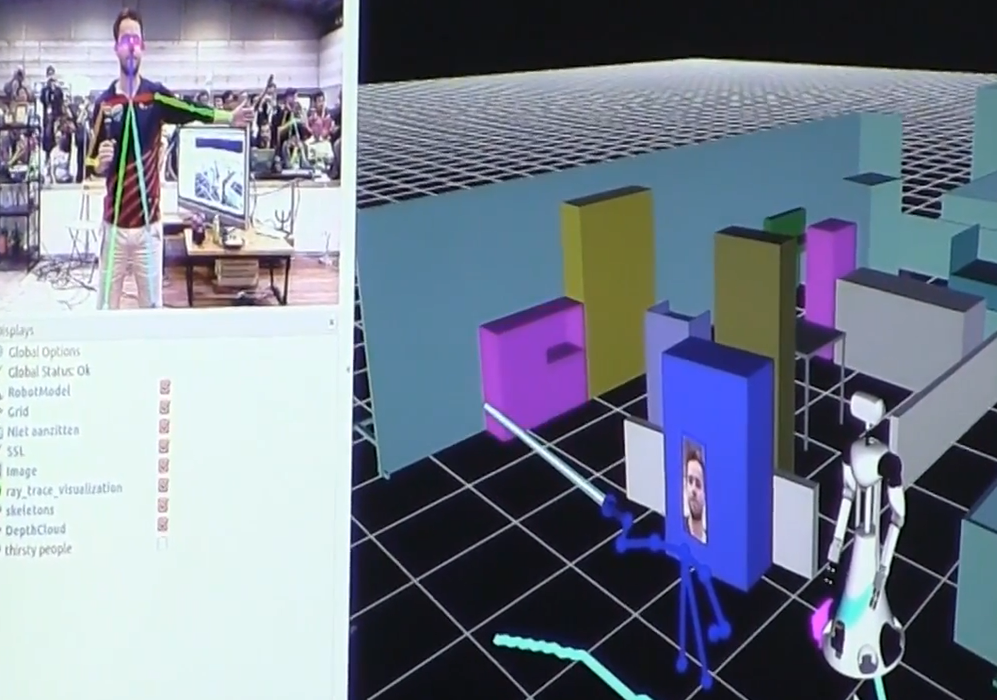
\includegraphics[width=0.6\linewidth]{ed_ray_trace2}
	\caption{Ray-tracing based on pose detection}
	\label{fig:ray_trace}
\end{figure}


